\begin{figure*}
  \centering
  \begin{subfigure}[b]{0.5\textwidth}
    \centering
    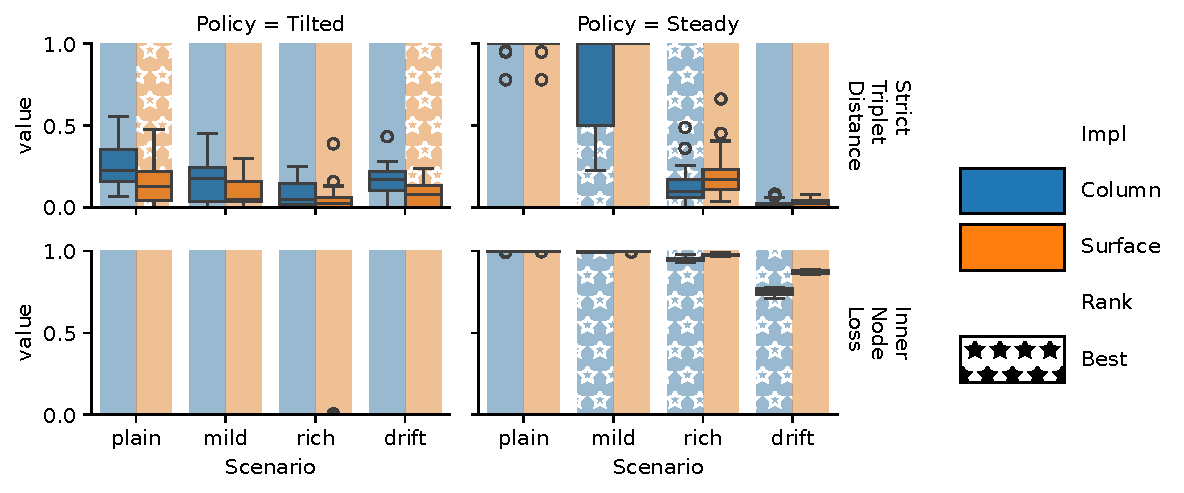
\includegraphics[width=\textwidth]{binder/binder/surf-vs-col/teeplots/annotation-size=64+col=policy+differentia-width=1+downsample=500+hue=impl+num-generations=100000+population-size=65536+row=variable+score=value+viz=peckplot+x=scenario+x-group=outer+y=value+ext=}
    \caption{Example reconstruction quality distributions. Lower is better.}
    \label{fig:col-vs-surf-example}
  \end{subfigure}%
  \begin{subfigure}[b]{0.5\textwidth}
    \centering
    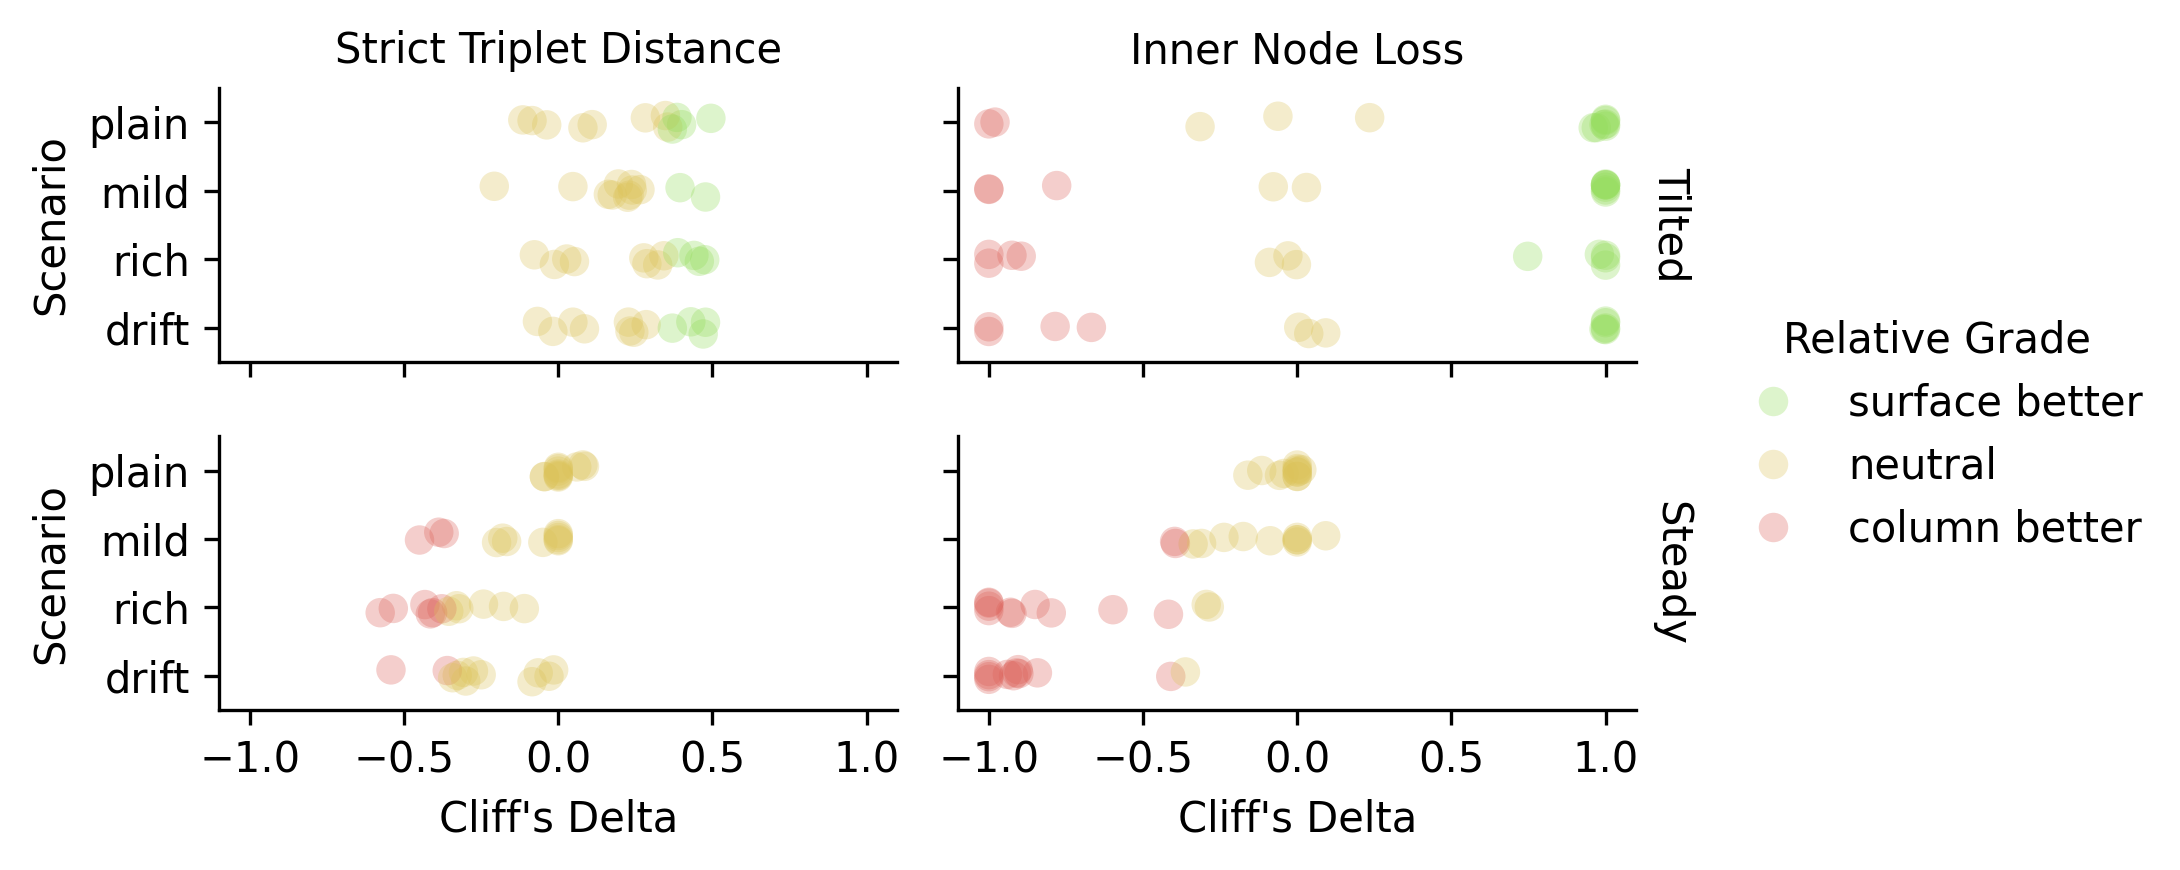
\includegraphics[width=\textwidth]{binder/binder/surf-vs-col/teeplots/col=metric+hue=relative-grade+kind=strip+row=policy+viz=catplot+x=cliff-s-delta+y=scenario+ext=}
    \caption{Reconstruction quality comparison outcomes.}
  \label{fig:col-vs-surf-overview}
  \end{subfigure}
  \caption{%
    \textbf{Does column- or surface-based instrumentation give higher-quality reconstruction?}
    \footnotesize
    Subpanel \ref{fig:col-vs-surf-overview} shows effect sizes of column-vs-surface comparisons for triplet distance and inner node loss metrics across sensitivity analysis conditions.
    Color coding indicates a significant outcome (Mann-Whitney U).
    Surface tends to outperform column under tilted policy and vice versa under steady policy.
    Subpanel \ref{fig:col-vs-surf-example} shows reconstruction quality effects for 64-bit size, bit-differentia annotations with population size 65,536, downsample size 500, and 100k generations.
    Background hatching indicates significant outcome.
    See Supplementary Figure \ref{fig:col-vs-surf} for listing of effects by sensitivity analysis condition.
  }
  \label{fig:col-vs-surf-summary}
\end{figure*}
